\documentclass[a4paper]{article}
\usepackage[utf8]{inputenc}
\usepackage{fancyhdr}
\usepackage[margin=2.5cm]{geometry}
\usepackage{amsmath, amssymb}
\usepackage{graphicx}

\fancyhf{}
% vspaces in den headern fuer Distanzen notwendig
% linke Seite: Namen der Abgabegruppe
\lhead{\textbf{Matthias Maile}\vspace{1.5cm}}
% rechte Seite: Modul, Gruppe, Semester
\rhead{\textbf{Höhere Mathematik 2\\Sommersemester 2020}\vspace{1.5cm}}
% Center: nr. des blattes
\chead{\vspace{2.5cm}\huge{\textbf{1. Übungsblatt}}}
% benoetigt damit der eigentliche Text nicht in der Überschrift steckt
\setlength{\headheight}{4cm} 


% eigene commands
\newcommand{\limxzer}{\lim_{x \rightarrow 0}}

\begin{document}
% pagestyle nicht global festgelegt, da sonst bei allen Seiten Überschrift ist
% daher muss hier fancy aktiviert werden (für eine Seite, daher thispagestyle)
\thispagestyle{fancy}

\section*{Aufgabe 1}
% ...
\[ f: (0,\infty) \rightarrow \mathbb{R}, f(x) = \frac{\ln x}{x} \]
Zu Beginn schon die ersten drei Ableitungen:
\[
	f^\prime (x) = \frac{1 - \ln x}{x^2} \qquad
	f^{\prime\prime} (x) =
	\frac{-3+2 \ln x}{x^3} \qquad
	f^{\prime\prime\prime} (x) =
	\frac{11 - 6 \ln x}{x^4}
	\]
\par{a)}
\begin{align*}
	\limxzer f(x) &= \limxzer \frac{\ln x}{x} = -\infty \\
	\lim_{x \rightarrow \infty} f(x) &= \lim_{x \rightarrow \infty} \frac{\ln x}{x} \\
	\text{Regel von l'Hospital} \Rightarrow &= \lim_{x \rightarrow \infty} \frac{\frac{1}{x}}{1} = \lim_{x \rightarrow \infty} \frac{1}{x} = 0
\end{align*}

\par{b)}
Damit wir mögliche Kandidaten für die Extremstellen von f erhalten benutze ich das notwendige Kriterium $f^\prime(x_0) = 0$:
\[ 
	f^\prime (x_0) = \frac{1-\ln x_0}{x_0^2} = 0 \Rightarrow 1-\ln x_0 =0
	\Rightarrow x_0 = e
\]
Zur Überprüfung wird das Hinreichende Kriterium $f^\prime (x_0) = 0, \ f^{\prime\prime}(x_0) \neq 0$ angewendet:
\[
	f^{\prime\prime} (x_0) = f^{\prime\prime} (x_0) = \frac{-3e + 2e*\ln e}{e^4} = -e^{-3}
	\]
durch einsetzen von $x_0 = e$ in die Funktion f erhalten die Position des Maximums:
\[
	f(x_0) = f(e) = \frac{\ln e}{e} = \frac{1}{e} > 0 > -\infty
	\]
da sich $f$ bei den Randstellen 0 bzw. $-\infty$ annähert, liegt bei $(e,f(e))$ ein globales Maximum.

\vspace{1cm}

\par{c)} Da $f^\prime$ stetig auf $(0,\infty)$ ist, können wir mit der Nullstelle aus b) und einsetzen von Werten im jeweiligen Intervall herausfinden:
\[
	x \in (0,e) \Rightarrow f^\prime(x) > 0 \qquad
	x = e \Rightarrow f^\prime(x) = 0 \qquad
	x \in (e,\infty) \Rightarrow f^\prime(x) < 0
\]
Daraus lässt sich direkt auf die Monotonie schließen:
\begin{align*}
	x \in (0,e) &\Rightarrow f \text{ streng monoton steigend} \\
	x \in (e,\infty) &\Rightarrow f \text{ streng monoton fallend}
\end{align*}
(Durch einschließen von e in den Intervallen wäre $f$ monoton fallend bzw. steigend.)

\newpage
\setlength{\headheight}{0cm} 

\par{d)} Für die Wendepunkte wird das notwendige Kriterium angewendet:
\begin{align*}
	f^{\prime\prime} (x_0)= 0 \Rightarrow \frac{-3+2 \ln x_0}{x_0^3} &= 0\\
	\Leftrightarrow \ln x_0 &= 1.5 \\
	\Leftrightarrow x_0 &= e^{1.5}
\end{align*}
Die Überprüfung mit dem hinreichenden Kriterium $f^{\prime\prime} (x_0) = 0, f^{(3)} \neq 0$:
\[ 
	f^{(3)} (x_0) = \frac{11 - 6*\ln(e^{1.5})}{e^{4*1.5}} = \frac{2}{e^6} \neq 0 
	\Longrightarrow (e^{1.5}, f(e^{1.5})) \text{ ist ein Wendepunkt}
\]
Da im intervall $(0,e^{1.5})$ ein Hochpunkt liegt, muss der Graph von $f$ auf dem Intervall konkav sein. Beim Wendepunkt ist die 3. Ableitung positiv. Die 1. Ableitung hat an der Stelle also einen Tiefpunkt, muss danach also wieder steigen. Somit ist $f$ für $x \in (e^{1.5}, \infty) $ konvex.
\begin{align*}
	x \in (0,e^{1.5}) &\Rightarrow f \text{ konkav} \\
	x \in (e^{1.5}, \infty) &\Rightarrow f \text{ konvex}
\end{align*}
\par{e)}
\begin{figure}[h]
	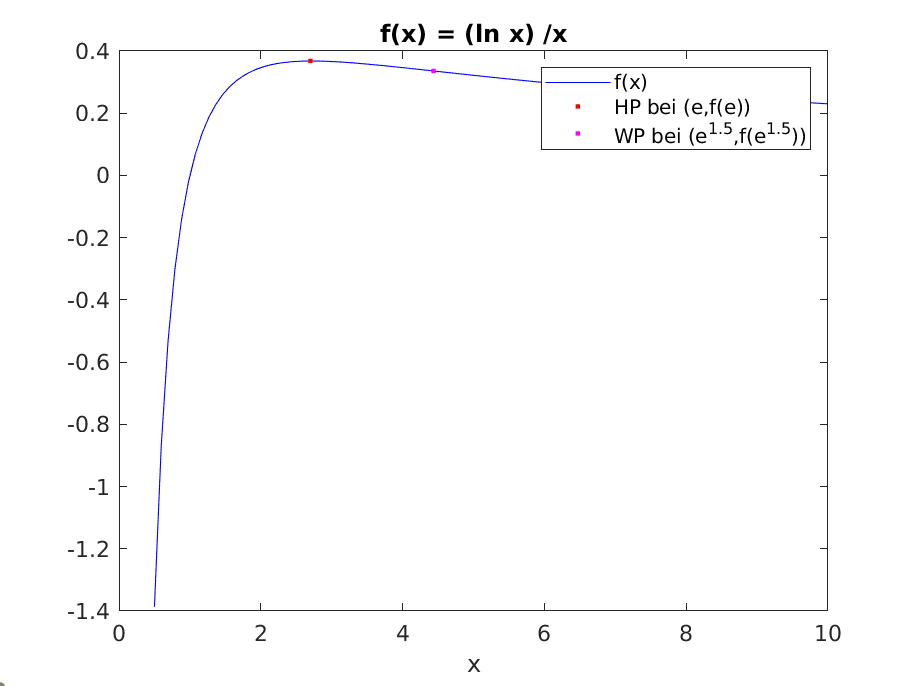
\includegraphics[width=15cm]{aufgabe1_plot.png}
\end{figure}
\newpage

\section*{Aufgabe 2}
% berechnung der ersten 4 taylor polynome bei x_0 = 1
\[ f: (0,\infty) \rightarrow \mathbb{R}, \quad f(x) = \ln(1 + \ln x) \]
aus Ketten- und Produktregel folgen die Ableitungen:
\begin{align*}
	f^\prime (x) &=
	\frac{1}{x (1+\ln x)} \\
	f^{\prime\prime} (x) &=
	\frac{-2 - \ln x}{x^2 * (1+\ln x)^2}\\
	f^{(3)} (x) &=
	\frac{2\ln^2\left(x\right)+7\ln\left(x\right)+7}{x^3\left(\ln\left(x\right)+1\right)^3} \\
	f^{(4)} (x) &=
	-\dfrac{6\ln^3\left(x\right)+29\ln^2\left(x\right)+52\ln\left(x\right)+35}{x^4\left(\ln\left(x\right)+1\right)^4} \\
	%f^{(5)} (x) &=
	%\dfrac{2\left(12\ln^4\left(x\right)+73\ln^3\left(x\right)+182\ln^2\left(x\right)+223\ln\left(x\right)+114\right)}{x^5\left(\ln\left(x\right)+1\right)^5}
\end{align*}
Das $n$-te Taylorpolynom am Entwicklungspunkt $x_0$ ist definiert durch
\[
	T_n(x;x_0) = \sum_{k=0}^n \frac{f^{(n)}(x_0)}{k!} (x-x_0)^k
	\]
Daraus ergibt sich bei der $f$ am Entwicklungspunkt $x_0 = 1$:
\begin{align*}
	T_0(x;1) &=
	f(1) = \ln (1 + \ln 1) = \ln 1 = 0 \\
	T_1(x;1) &=
	T_0(x;1) + f^\prime(1) * (x-1) = 0 + (x-1) * 1 = x - 1 \\
	T_2(x;1) &=
	T_1(x;1) + \frac{f^{\prime\prime}(1)}{2} * (x-1)^2 = x - 1 + (-1) * (x^2 - 2x + 1) = -x^2 + 3x -2 \\
	T_3(x;1) &=
	T_2(x;1) + \frac{f^{(3)}(1)}{6} * (x-1)^3 = -x^2 + 3x -2 + \frac{7}{6} * (x-1)^3 
	% -x^2 + 3x - 2 + 7/6 (x^3 - 3x^2 + 3x -1) = -x^2 + 3x - 2 + 7/6 x^3 - 7/2 x^2 + 7/2 x - 7/6
	= \frac{7}{6} x^3 - \frac{9}{2} x^2 + \frac{13}{2} x - \frac{19}{6}
\end{align*}
Das Restglied von Lagrange lautet nach der Taylorschen Formel:
\begin{align*}
	R_n(x,x_0) :	&= \frac{f^{(n+1)}(\xi)}{(n + 1)!} (x - x_0)^{n+1} \\
	\Rightarrow R_3(x,1) &= \frac{f^{(4)}(\xi)}{24} * (x-1)^4  \\
	&= -\dfrac{6\ln^3\left(\xi\right)+29\ln^2\left(\xi\right)+52\ln\left(\xi\right)+35}{\xi^4\left(\ln\left(\xi\right)+1\right)^4} * \frac{(x-1)^4}{24}
\end{align*}
mit einer Stelle $\xi = x_0 + \alpha(x-x_0)$ und $\alpha \in (0,1)$.

\end{document}
